\chapter{Grid generation}\label{cha:grid-gen}
In this chapter we discuss methods that allows us to apply our prior knowledge directly into the grid generation process.
This is a stark contrast to the methods in the previous chapter, where we imposed our constraints in the learning process.
Even though these methods work well even with limited prior knowledge, they have one major drawback:
We \emph{always} have to generate a complete sparse grid.
This was not a problem for low to mid-dimensional datasets, but is a limiting factor for higher dimensional problems.
\sidetitle{High dimensional problems}
To tackle very-high dimensional problems, we need to be able to influence the
grid generation.

We will discuss two modifications of the grid generation algorithm in this
chapter.
The first one, generalized sparse grids, allows us to create grids with variable granularity.
The second method, interaction-term aware sparse grids, use knowledge about the
importance of interaction-terms to create grids that are both smaller and more effective.
\section{Generalized Sparse Grids}\label{sec:generalised-sg}
Generalized sparse grids allow us to create grids with a variable granularity.
They can be used to create smaller grids while retaining the approximation
error, given some additional smoothness constraints.
They were first developed by \citeauthor{optimizedApproxSpaces} in~\cite{optimizedApproxSpaces}.
A discussion about their usefulness for machine learning can be found
in~\cite{sparse-reconstruction} and in~\cite{sparse-parsimony}.

\subsection{Theory}
Despite the fact that the generalised sparse grid technique originates from
an elaborate functional analysis argument, they can be stated by two simple formulas.
We only need to change \cref{eq:sparse-grid-space} to generalize our grid.
The set of grid points for the generalized sparse grid \(G^T_n\) of level \(n\)
and its corresponding approximation space \(V^T_n\) is described by
\begin{align}\label{eq:generalised-grid-space}
G_n^T &= \bigcup_{\mathclap{\substack{\vert {\bm{l}} \vert_1 - T \vert \bm{i} \vert_\infty \\ \leq n + d - 1 - T n}}} G_{\bm{l}},\\
V_n^T &= \bigoplus_{\mathclap{\substack{\vert {\bm{l}} \vert_1 - T \vert \bm{i} \vert_\infty \\ \leq n + d - 1 - T n}}} W_{\bm{l}}.\nonumber
\end{align}
The constant \(T\) chosen in the interval \((-\infty, 1]\) governs our choice of
sub-spaces and thus also the granularity of the grid.
Setting \(T\) to zero recovers the standard sparse grid, higher values
approaching one transform the grid to the form seen in \cref{fig:grids-T-1}.
The limit \(T \to -\infty\) corresponds to a full grid.
Note that even though the value of \(T\) is continuous, it acts as a discrete operator.
This is why the actual value of \(T\) does not matter, different values can result in the
same grid.
An example for a two-dimensional grid with level four can be seen in \cref{fig:grids-T}.
\begin{figure}[H]
  \centering
  \begin{subfigure}[b]{0.23\textwidth}
    \centering
    \includegraphics[width=\textwidth]{{{grid_T-inf}}}
    \caption{\(T = -\infty\)}
  \end{subfigure}
   \begin{subfigure}[b]{0.23\textwidth}
    \centering
    \includegraphics[width=\textwidth]{{{grid_T0}}}
    \caption{\(T = 0.0\)}
  \end{subfigure}
 \begin{subfigure}[b]{0.23\textwidth}
    \centering
    \includegraphics[width=\textwidth]{{{grid_T0.5}}}
    \caption{\(T = 0.5\)}
  \end{subfigure}
 \begin{subfigure}[b]{0.23\textwidth}
    \centering
    \includegraphics[width=\textwidth]{{{grid_T1.0}}}
    \caption{\(T = 1.0\)}\label{fig:grids-T-1}
  \end{subfigure}
  \caption{Grid visualization for 2-dimensional grids with different \(T\)s}\label{fig:grids-T}
\end{figure}
The dimension of a generalized sparse grid with level \(n\) and constant \(T\) can be described by
\begin{equation*}
  \operatorname{dim}(V^T_n) \leq
  \begin{cases}
    d 2^n & T = 1, \\
    \BigO(2^n) & T \in (1/n, 1),\\
    \BigO(2^n n^{d-1}) & T \in [0, 1/n],\\
    \BigO(2^{\frac{T - 1}{T/d - 1} n}) & T < 0.
  \end{cases}
\end{equation*}
We can see that the special cases \(T = 0\) and \(T \to \infty\) are covered~\cite{optimizedApproxSpaces}.
While it is possible to state a formula for the approximation error it is quite hard to
apply it to machine learning problems, as the smoothness properties of real world
datasets are unknown.
This means that it is hard to decide, whether generalized sparse grids make
sense for a given problem, without generating a model.
We can view the generalized sparse grids from a different perspective as well.
A higher value of \(T\) decreases the amount of higher-order interaction terms,
without decreasing the number of basis functions that model only one variable.
The effect for a grid with dimension 4 and level 5 can be seen in \cref{fig:interaction-T}.
\begin{figure}[thb]
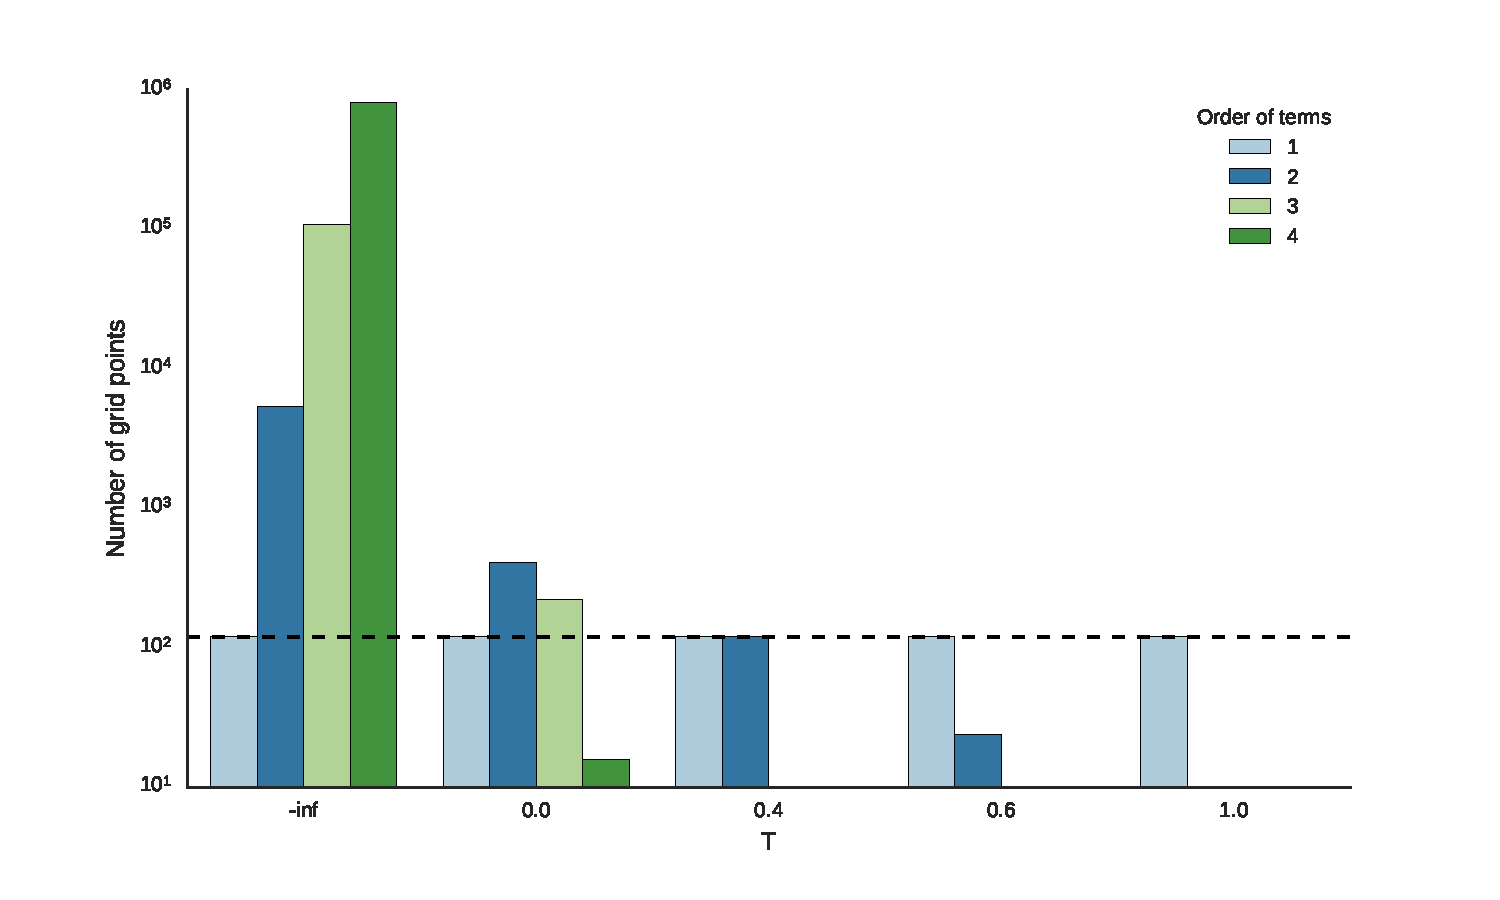
\includegraphics{interactionT}
\caption{Number of terms of each order for a grid with dimension 4 and level 5.
The bias term is not included in the graphic, it is contained in all grids.}\label{fig:interaction-T}
\end{figure}
Note that the grid for \(T = 1\) does not contain any interaction terms.
Smaller values of \(T\) increase the number of interaction terms, until the full
grid is reached.
  Because the importance of feature interactions is hard to judge for most problems, this heuristic is also difficult to apply.

\subsection{Implementation}
The implementation is quite simple.
It was possible to change the already existing grid generation algorithm, to include the changed inclusion criterion described by \cref{eq:generalised-grid-space}.
\begin{algorithm}[h]
 \caption{Generalised Sparse Grid Generation}\label{alg:gen-sg} 
 \begin{algorithmic}[1]
   \Require{Number of dimensions and level \(n\)}
   \Statex
   \Function{GridGeneration}{dimensions, $n$}
   \For{\(0 \leq d < \text{ dimensions}\)}
   \State\Call{CreatePoint}{d, 1, 1} \Comment{Bias points}
   \EndFor
   \For{\((l, i) \in \{(l,i) \, \mid 1 \leq l \leq n \land 1 \leq i < l^2,\, i \text{ odd} \} \)}
     \State\Call{CreatePoint}{0, l, i} \Comment{1d-grid points for first dimension}
   \EndFor
   \For{\( d < \text{dimensions}\)}
   \For{\(p \in \Call{GetAllGridPoints}{}\)}
   \Let{levelSum}{\Call{p.getLevelSum}{} - 1}
   \Let{levelMax}{\Call{p.getLevelMax}{}}
   \Let{l}{1}
   \While{\(\max(l, \text{levelMax}) \leq n\)}
   \Let{left}{\((l + \text{ levelSum}) - (T \cdot \max(l, \text{ levelMax})) \)}
   \Let{right}{\((n + \text{ dimensions} - 1) - (T \cdot n)\)}
   \If{left \(>\) right}
   \State\Call{break}{}
   \EndIf
   \For{\(1 \leq i < 2^l, i \text{ odd}\)}
   \State\Call{CreatePointAt}{d, l, i, p}
   \EndFor
   \Let{l}{l + 1}
   \EndWhile
   
   \EndFor
   \EndFor
   \EndFunction
 \end{algorithmic}
\end{algorithm}
The resulting algorithm is given by \cref{alg:gen-sg}, lines 11--13 correspond to our changes.
We use the functions \textsc{CreatePoint}, which generates a point for a given
level and index, and \textsc{CreatePointAt}, which also generates a point, but
this time as a child of another point.
For the discussion here the distinction is not important, because our algorithms do not rely on the hierarchical structure of the grid.
Our implementation is a direct translation of the pseudo-code.
\subsection{Results \textit{\&} Discussion}
\newenvironment{ttable}{
  \begin{tabular}[c]{S[table-format=2.1]
    S[table-format=1.4, table-figures-exponent=2, table-sign-mantissa, table-sign-exponent]
    S[table-format=4.1(4)]
    S[table-format=2.1]
    c
    c
    S[table-format=2.3]
    S[table-format=2.3]}
  \toprule \multicolumn{1}{c}{\(T\)}
& \multicolumn{1}{c}{\(\lambda\)}
& \multicolumn{1}{c}{\textsc{cv}-Grid}
& \multicolumn{1}{c}{\textsc{cv-rmse}}
& \multicolumn{1}{c}{Train-Grid}
& \multicolumn{1}{c}{Train-\textsc{rmse}}
& \multicolumn{1}{r}{Test-\textsc{rmse}}
\\\midrule}{\bottomrule\end{tabular}}

Generalized grids work well in theory.
To show their practical performance, we tested two things that we will discuss
in this section:
\begin{enumerate}
\item In what way does the grid parameter \(T\) influence the regularization
  parameter \(\lambda\)?
\item Can we archive a better performance with generalised sparse grids compared
  to standard grids, with a comparable number of grid points?
\end{enumerate}
\todo{Train-Grid should be an integer!}
\begin{table}[tb]
    \begin{ttable}
-0.5 & 2.2762e-10 & 5541.3( 185) & 1.246 & 5547.0 & 0.823 & 1.226\\
0 & 1.4539e-04 & 2278.8(  33) & 1.196 & 2277.0 & 0.845 & 1.179\\
0.5 & 7.7081e-05 & 640.8( 141) & 1.051 & 651.0 & 0.959 & 1.028\\
1 & 1.0432e-04 & 391.2(  72) & 1.031 & 395.0 & 0.976 & 1.015\\
    \end{ttable}
\caption[T vs \(\lambda\) for friedman1 dataset.]{Best results and used \(\lambda\) for different
  \(T\)s for the Friedman1 dataset and an estimator with level
  four.
  The \textsc{cv}-Grid size is reported with its standard deviation.}\label{fig:t-vs-mse-friedman1}
\end{table}

\sidetitle{Friedman1}
We performed 25 iterations of a Bayesian hyper-parameter search for \(\lambda\) for the Friedman1 dataset with identity regularization and a generalized sparse grid for different \(T\)s and level four.
Each learner performed five adaptivity steps refining three points each.
The results can be seen in \cref{fig:t-vs-mse-friedman1}.
In this case, the best results were archived for \(T = 1\) and the smallest grid
size, all other parameters overfit the data.
This happens because we used a small version of the Friedman1 dataset---it
being an artificially created dataset, it would be easy to create more samples
and then fit an arbitrarily large model.
We can see from this example, that generalised sparse grids allow us to use a
higher level, which corresponds to a larger amount of grid points with order
one, than with standard sparse grids.
Additionally the combination with adaptivity allowed us to start with an
estimator that only models few interaction terms and then creating needed
interaction points on demand.
The parameter \(\lambda\) describes the amount of regularization per
grid point.
We can see no trend in the results for the Friedman1 dataset for \(\lambda\).
Only the value for \(T = -0.5\) is smaller by some orders of magnitude.
A possible reason for that might be the same reason the sparse grid with \(T =
1\) showed the best result:
Except for the \((x_1 \times x_2)\) interaction, the Friedman1 dataset has no
qualitative interactions, i.e.~interactions that are inherently additive in effect.
This implies that the additional interaction points for larger grids would
have a rather low surplus, even for an estimator fit without regularization.
The higher-order grid points thus need a smaller amount of regularization than
the first-order terms, which explains the small \(\lambda\) for the largest
grid.
All other regularization parameters have values that are of similar order, the
differences do not seem to be significant.
The Friedman1 results demonstrated that generalized grids can help us to use
grids with a level, that would lead to severe overfitting for normal sparse
grids.

\begin{table}[tb]
    \begin{ttable}
-0.4 & 1.9276e-02 & 8468.7( 206) & 4.703 & 8470.0 & 2.275 & 4.215\\
0 & 1.9622e-02 & 6678.3( 271) & 4.709 & 6650.0 & 2.286 & 4.184\\
0.5 & 6.2935e-03 & 1140.4( 239) & 4.771 & 1180.0 & 2.664 & 3.797\\
0.6 & 1.2700e-02 & 712.7( 242) & 4.781 & 685.0 & 3.398 & 4.308\\
    \end{ttable}
\caption[T vs \(\lambda\) for concrete dataset.]{Best results and used \(\lambda\) for different
  \(T\)s for the concrete dataset and an estimator with level five. The optimal
  \textsc{rmse} is 1.0.}\label{fig:t-vs-mse-concrete}
\end{table}

\sidetitle{Concrete}
We used a similar experiment for the concrete dataset, this time performing 45
Bayesian search iterations and using estimators with level five.
For this dataset the chosen level did not lead to overfitting even for the
highest value of \(T\) and we can therefore use it to discuss the trade-off
between approximation accuracy and grid size our proposed method makes.
The results can be seen in \cref{fig:t-vs-mse-concrete}.
Note that there is a correlation between grid size and the errors: larger grids
perform better, at least for the cross validation and training error metrics.
A further increase of the level of the approximation space could soon lead to overfitting.
Even for our chosen level, we have more grid points than training examples in the \(T \geq 0.5\) cases , which leads to an underdetermined linear system.
We can also see that the decrease in error between the largest grid and the standard sparse grid is rather small, considering the amount of additional grid points needed.
Note that the estimator with \(T = 0\) has a higher \textsc{cv}- and
train-\textsc{rmse} than the learner with \(T = -0.4\), but a lower testing
error.
This and the fact that the differences are small lead to results for which it is
hard to decide, which choice of \(T\) performed best.
Because of that we can see that the trade-off between error and discretization cost, which the generalized sparse grids make, works.
They used fewer grid points to achieve similar errors.

If we compare the performance of the generalised sparse grid with level five and
\(T = 0.5\) with the standard sparse grid of level four with the same adaptivity
settings, we can see that the generalised grid performs better than the standard grid, even though they both
use a similar number of grid points.
The standard grid with level four needed 1470 gridpoints for a \textsc{cv-rmse}
of 5.007, which means that it needed more grid points for a worse performance.

\begin{figure}[htb]
  \centering
  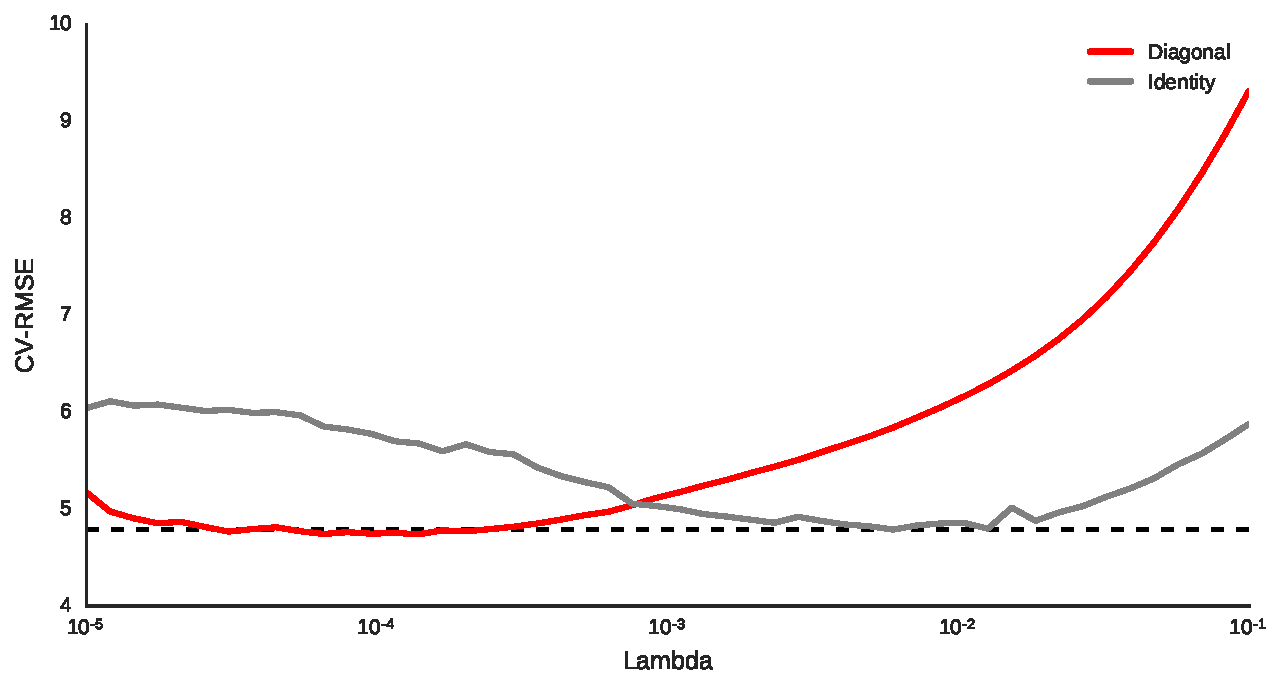
\includegraphics[width=\textwidth]{tikhonov_concrete_l5}
  \caption{This figure presents the obtained results for the concrete dataset
    obtained with estimators with level five and \(T = 0.5\).}
  \label{fig:tikhonov-concrete-l5}
\end{figure}

\todo{Maybe compare the minimums of both quickly?}
As an additional result, generalized sparse grids combined with the diagonal
matrix regularization functional show further potential.
An example for this can be seen in \cref{fig:tikhonov-concrete-l5}, which depicts a grid search
similar to the one in \cref{sec:tikh-discussion}, only using a level five grid
with \(T = 0.5\) instead of a level four grid with \(T = 0\).

We can conclude that our proposed method can improve the performance without additional cost.
Because the smoothness constraints for the generalized grids are stronger than the assumptions of the standard grid, this result does not have to hold for all datasets.
Even though its performance depends on the relevance of the higher-order-terms, it is hard to predict whether our proposed method will show good results.
The reason for this is that it is difficult to tell if interactions are relevant for a given dataset in the general case.
Therefore it seems useful and necessary, to build multiple models with different grid types and thus include the granularity of the grid into the model selection process.

\section{Interaction-Term Aware Sparse Grids}
As previously noted, sparse grids not only include grid points, which model an original feature, but
also interaction points.
We have seen that sparsity-inducing penalties perform automatic feature
selection.
In some cases we are able to make an educated guess which interactions are
relevant before actually training a model.
We will introduce a method in this section that allows us to create
interaction-term aware sparse grids, i.e.~grids that only contain a subset of
all possible interaction terms.
We will also present an application for this method: image recognition.
A discussion of this method can be found in \cite{sparse-parsimony}.

\subsection{Theory}
\sidetitle{No.~ of Interaction Terms}
We can calculate the number of included terms for a \(d\)-dimensional dataset
discretized using a sparse grid of level \(l\) using simple combinatorics:
\begin{equation*}
  \operatorname{count-terms}(d, l) = \sum_{k  = 0}^{\max (d, l-1)} \binom{d}{k}.
\end{equation*}
Because the number of grid points is directly related to the number of chosen
interaction terms, it is clear that the standard sparse grid technique become
computationally expensive or infeasible for very high dimensional problems.
This means that we have to restrict ourselves to a small level and are therefore
limited to low-order terms.
If we only interactions between some variables we can use larger levels without increasing the number of interaction terms to an intractable number.

\sidetitle{Nearest Neighbors}
An example where this technique is useful is image recognition.
Assume we have a 2-dimensional picture, where each pixel corresponds to a feature.
We make the following assumption:
Interactions between pixels that are close to each other spatially are more
important than interactions between pixels that are further away from each
other.
They are more important because they are likely to reveal the structure of the image.

Let \(d\) be a metric that measures the distance between two pixels.
Examples for widely-used metrics are
\begin{align*}
  d{(\bm{a}, \bm{b})}_{\Vert \cdot \Vert_2} &= \sqrt{(a_1 - b_1)^2 + (a_2 - b_2)^2},\\
  d{(\bm{a}, \bm{b})}_{\Vert \cdot \Vert_1} &= \vert a_1 - b_1 \vert + \vert a_2 - b_2 \vert,
\end{align*}
which are called the Euclidean and the Manhattan distance respectively.
We can then calculate the nearest neighbors of each pixel by iterating over all
other pixels and checking whether the metric is below a certain threshold.
To calculate all neighbors we simply iterate over each pixel.
This is not an asymptotically optimal algorithm, we pay \(\BigO(n^2)\) for all
features.
Even though more efficient algorithms exist, our method is good enough, because
we only have to calculate the neighbors once per dataset which is negligible
compared to the cost of training the actual model.
After calculating the neighbors, we can generate the interactions from them.
They are given by all \(i \leq \max(d, l-1)\) long combinations of all possible
neighbors for each pixel, where \(i\) is an arbitrarily chosen value.
This means that it is possible, to create grids with a high level without some
higher-order terms.
For example, it is possible to create a grid with level six, but only use the
interactions up to order four.
In fact, it is useful to start with a low-level grid but to use higher-order interaction terms during refinement.
This recovers the usual behavior of non-interaction-term aware sparse grids.

\begin{figure}[hbt]
  \centering
  \begin{subfigure}[b]{0.4\textwidth}
    \centering
    \includegraphics{{{nn_l1}}}
    \caption{\(d{(\bm{a}, \bm{b})}_{\Vert \cdot \Vert_2} \leq 2\)}
  \end{subfigure}
  ~
   \begin{subfigure}[b]{0.4\textwidth}
    \centering
    \includegraphics{{{nn_l2}}}
    \caption{\(d{(\bm{a}, \bm{b})}_{\Vert \cdot \Vert_1} \leq \sqrt{2}\)}
  \end{subfigure}
  \caption{Nearest Neighbors for two different metrics. The darkest point is the
  origin, the other colored points are its neighbors.}\label{fig:neighbors-cmp}
\end{figure}

\begin{algorithm}[h]
  \caption{Nearest Neigbors}\label{alg:neigbors}
  \begin{algorithmic}[1]
    \Require{Set of all pixels \(p\), distance metric \(d \from (\mathbb{R}^2, \mathbb{R}^2) \to \mathbb{R}\), threshold \(t\) }
    \Statex
    \Function{NearestNeighbors}{$p, d, t$}
    \Let{neighbors}{vector<vector<int>>()}
    \For{\(a \in p\)}
      \For{\(b \in p\)} \Comment{Each pixel is its own neighbor in our case.}
      \If{\(d(a,b) \leq t\)}
      \State\Call{append}{curNeighbors, y}
      \EndIf
      \EndFor
    \State\Call{append}{neighbors, curNeighbors}
    \EndFor
    \State\Return{neighbors}
    \EndFunction
  \end{algorithmic}
\end{algorithm}

\subsection{Implementation}
Similar to the implementation of the generalised sparse grids we need to
make some small adjustments to the grid generation algorithm described in \cref{alg:gen-sg}.
We pass an additional parameter to the function \textsc{GridGeneration} that determines the interaction terms we want to integrate into the model.
This parameter is a list of interactions, each interaction is modelled as a list of dimensions that should interact with each other.
The list is then converted to a hash set that stores one boolean vector for each interaction.
Each entry of this vector is true if the dimension should be used and false otherwise.
For example a \((x_1 \times x_2)\) interaction for a 3-dimensional dataset is
modelled as the vector \((1, 2)\) and the corresponding boolean vector is then given by (\emph{true}, \emph{true}, \emph{false}).

We then only need to modify the function \textsc{createPointAt} (called in line 17).
Before creating the grid point, we check if the new grid point models a desired
interaction.
Each possible new point is encoded in the same manner as the interactions, as a
boolean vector that indicates the used dimensions.
The decision, whether a grid point should be included amounts to a simple check,
if the possible new dimension-combination is contained in the aforementioned
hash set.

We have to make the same adjustments to the adaptivity procedure.
Our implementations is simple, because we leverage the existing adaptivity
procedure of the \textsc{sgpp} implementation.
We implemented a class HashRefefinementInteraction that inherits from the base
class HashRefinement.
This base class implements the actual refinement procedure, the subclass leaves
all but one function unchanged.
The function \textsc{createGridPoint} is called to create the new grid points.
We modify this function in a straight forward way:
Before each point is added to the model, we perform the same check as in the
method \textsc{createPointAt}.

This implementation strategy is efficient due to the underlying implementations.
It costs us \(\BigO(1)\) operations to check if an element is contained in the set, which is both asymptotically optimal and efficient in practice.
The boolean vector in the \emph{C++} standard library is implemented as a
bitfield, which results in a lower space overhead.

\subsection{Results \textit{\&} Discussion}
To check the validity of the interaction-term aware sparse grids and of the
nearest neighbor approach for images, we use a version of the classical \textsc{mnist}-dataset, obtained from the
\textsc{uci} machine learning repository~\cite{datasets-uci}.
The goal of this dataset is to use hand drawn pictures of one digit each to
classify the digit depicted.
\begin{figure}[htb]
  \centering
  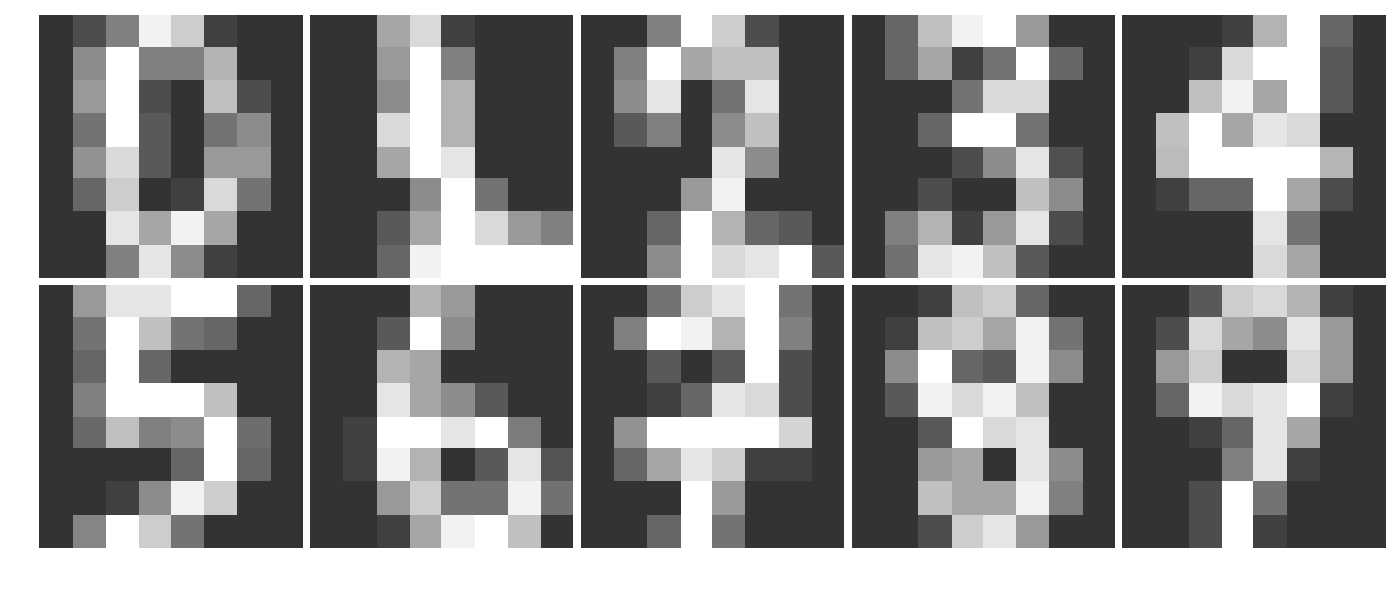
\includegraphics[width=\textwidth]{optdigits}
  \caption{Some examples for digits}
  \label{fig:optdigit-images}
\end{figure}
Our version of the dataset is composed of 64-features, each one represents one
gray-scale pixel in the range 0--15.
Trying to construct a sparse grid for such a highly dimensional dataset is
possible for small levels and becomes highly intractable for larger levels.
This is why we need to exclude most of the interaction terms.
We used algorithm xxx to select the neighbors for each pixel, and only include
the nearest neighbors in our grid.
This was done using the Euclidean distance with a threshold of \(\sqrt{2}\),
which leads to a \(3 \times 3\) convolution.
An example of this can be seen in figure xx.
The effect on the grid sizes for some different metrics are shown in table xxx.

\begin{figure}[htb]
  \centering
  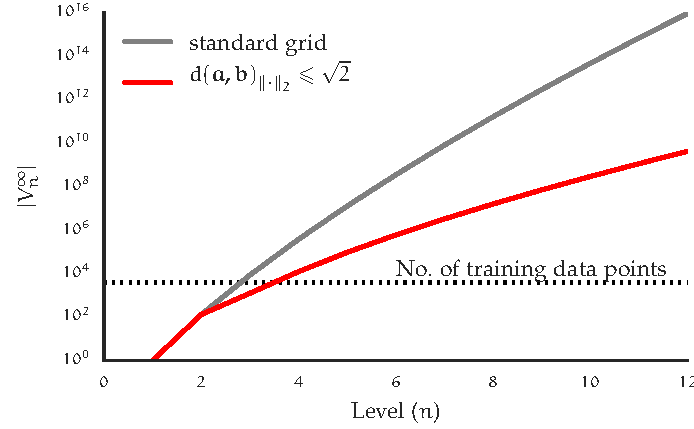
\includegraphics{interaction_sizes}
  \caption{Comparison of grid sizes with standard and interaction-term aware
    sparse grids for the optical digits dataset.}
  \label{fig:optdigit-gridsize}
\end{figure}

\todo{Use full dataset for tsne plot!}
\begin{figure}[htb]
  \centering
  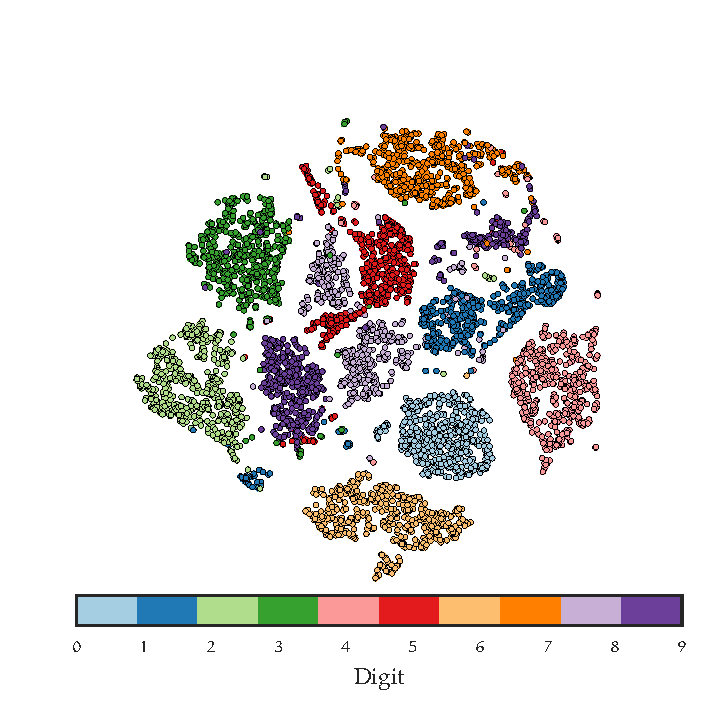
\includegraphics[width=\textwidth]{tsne_optdigits}
  \caption{\textsc{T-sne} plot of the optdigits dataset}
  \label{fig:optdigit-tsne}
\end{figure}

\sidetitle{Estimating \(\lambda\)}
Because we have to train one regression learner for each class it takes a rather
long time to generate a model, which in practice meant that a grid search for
the regularization parameter was infeasible.
This is why we tried to find an approximation by using only a three-class subset
of the dataset for this purpose.
The smaller dataset comes with two advantages.
Firstly we only had to use three regression models for each classification
task and secondly the training of each model was considerably faster, because
the sparse grid model scales linearly with the number of training points.
The downside is of course that the estimated best \(\lambda\) is only a crude
approximation of the optimal one.
Because our model assumes that each binary sub-classification model uses the
same hyper-parameters there is some variance of the best-parameter to consider.
The discrete nature of the decision problem also allows us some leeway.
Altogether our approximation of the hyper-parameter might not be entirely
optimal, but it should be good enough.
Finally we performed a grid search for \(\lambda\) using a ridge regularized model with level
three and the aforementioned choice of interaction terms.
We used a three-fold stratified cross validation metric to compare the models.
The best learner achieved an \textsc{cv}-accuracy of 100\% on this subset with
\(\lambda = 0.1\).
Of course, this is not a good estimate for the error on the complete dataset,
but still delivers a solid estimate for the regularization parameter.
The results also showed that the choice of \(\lambda\) does not influence the
validation accuracy heavily as a learner with \(\lambda = 10^{-12}\) achieved a
\textsc{cv}-accuracy of about 99.91.

\sidetitle{Final Model}
Using our approximated best regularization parameter we then created two models,
one using no adaptivity and one, where we performed two adaptivity steps
refining ten points each.
The results of our learners and some other models can be seen in table xxx.
We can see that we achieved better results using the interaction-terms aware
sparse grids than the adaptive sparse grid estimator of \cite{spatAdaptGrid},
even without using refinement ourselves.
Combining our proposed grid generation scheme with adaptivity allowed us to
further improve our results, \ldots.

We can see, that the usage of knowledge about the structure of images can help
us considerably by using grind-points with higher information content.
Another effect of our proposed method is that we can use a higher level, because
we exclude many interaction terms.
This results in grids that achieve competitive results compared to more costly
adaptive grids.

%%% Local Variables:
%%% mode: latex
%%% TeX-master: "../main"
%%% End:
